\documentclass[10pt,a4paper]{article}
\usepackage[utf8]{inputenc}
\usepackage[margin=1in]{geometry}
\usepackage{xcolor}
\usepackage{graphicx}
\usepackage{titlesec}
\usepackage{enumitem}
\usepackage{hyperref}
\usepackage{amsmath}
\usepackage{listings}
\usepackage{tikz}
\usetikzlibrary{shapes,arrows,positioning}

% Color scheme
\definecolor{primary}{RGB}{41,128,185}
\definecolor{secondary}{RGB}{52,152,219}
\definecolor{accent}{RGB}{231,76,60}
\definecolor{lightgray}{RGB}{245,245,245}
\definecolor{darkgray}{RGB}{51,51,51}

% Custom section formatting
\titleformat{\section}
  {\normalfont\Large\bfseries\color{primary}}
  {\thesection}{1em}{}

\titleformat{\subsection}
  {\normalfont\large\bfseries\color{secondary}}
  {\thesubsection}{1em}{}

% List styling
\setlist[itemize]{leftmargin=*,itemsep=0.1cm,topsep=0.2cm}
\setlist[enumerate]{leftmargin=*,itemsep=0.1cm,topsep=0.2cm}

% Code listing style
\lstset{
    basicstyle=\ttfamily\small,
    breaklines=true,
    frame=single,
    backgroundcolor=\color{lightgray},
    rulecolor=\color{darkgray},
    numbers=left,
    numberstyle=\tiny\color{darkgray},
    keywordstyle=\color{primary},
    commentstyle=\color{gray},
    stringstyle=\color{accent},
}

% Header and footer
\usepackage{fancyhdr}
\pagestyle{fancy}
\fancyhf{}
\rhead{\color{darkgray}\thepage}
\lhead{\color{darkgray}\leftmark}
\renewcommand{\headrulewidth}{0pt}

% Project title command
\newcommand{\projecttitle}[1]{
    \begin{center}
        {\Huge\bfseries\color{primary} #1}\\
        \vspace{0.5cm}
        \textcolor{darkgray}{\large Project Documentation}
    \end{center}
}

\begin{document}

% Title Page
\begin{titlepage}
	\centering
	\vspace*{2cm}

	\projecttitle{Ouroboros}

	\vspace{1cm}

	\includegraphics[width=0.5\textwidth]{project-logo.png} % Replace with your project logo

	\vspace{1cm}
	\begin{center}
		\href{https://github.com/Kaya-Sem/ouroboros}{
\includegraphics[width=0.1\textwidth]{images/github-mark.png}}
	\end{center}

	\vspace{1cm}

	\textcolor{darkgray}{\large Kaya-Sem Van Cauwenberghe}\\
	\textcolor{darkgray}{\today}

	\vfill

	\begin{abstract}
		\noindent
		\textcolor{darkgray}{A concise summary of the project, its purpose, and key achievements. This should be 3-5 sentences that capture the essence of what makes this project noteworthy.}
	\end{abstract}

	\vspace{1cm}

	\small
	\textcolor{darkgray}{Document version: 1.0}
\end{titlepage}

\tableofcontents
\newpage

\section{Project Overview}
\subsection{Introduction}
Brief introduction to the project, its purpose, and the problem it solves. Explain the motivation behind the project and its core objectives.

\subsection{Key Features}
\begin{itemize}
	\item Feature 1 with brief description
	\item Feature 2 with brief description
	\item Feature 3 with brief description
	\item Feature 4 with brief description
\end{itemize}

\section{Technologies Used}
\subsection{Core Technologies}
\begin{itemize}
	\item \textbf{Programming Language(s)}: Go
	\item \textbf{Frameworks \& Libraries}: Key frameworks and libraries
	\item \textbf{Tools}: Development tools, CI/CD, etc. Docker, Docker-Compose
	\item \textbf{Infrastructure}: Hosting, databases, etc.
\end{itemize}

\subsection{Technology Diagram}
\begin{center}
	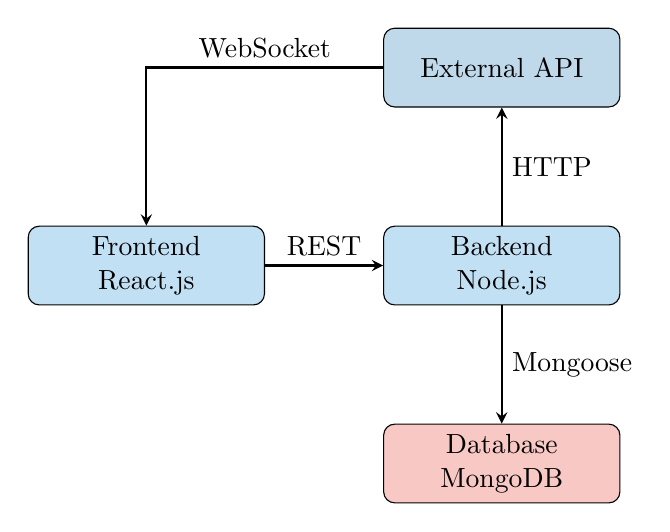
\begin{tikzpicture}[
			node distance=1.5cm,
			box/.style={draw, rounded corners, fill=lightgray, minimum width=3cm, minimum height=1cm, align=center},
			arrow/.style={->, >=stealth, thick}
		]

		\node[box, fill=secondary!30] (frontend) {Frontend\\React.js};
		\node[box, fill=secondary!30, right=of frontend] (backend) {Backend\\Node.js};
		\node[box, fill=accent!30, below=of backend] (database) {Database\\MongoDB};
		\node[box, fill=primary!30, above=of backend] (api) {External API};

		\draw[arrow] (frontend) -- (backend) node[midway, above] {REST};
		\draw[arrow] (backend) -- (database) node[midway, right] {Mongoose};
		\draw[arrow] (backend) -- (api) node[midway, right] {HTTP};
		\draw[arrow] (api) -| (frontend) node[near start, above] {WebSocket};

	\end{tikzpicture}
\end{center}

\section{Technical Details}
\subsection{Architecture}
Detailed explanation of the system architecture. Include subsections as needed for different components.

\subsection{Data Flow}
Description of how data moves through the system. You can include another diagram here if helpful.

\subsection{Key Algorithms}
If your project involves interesting algorithms or technical solutions, describe them here.

\begin{lstlisting}[language=Python,caption=Sample code snippet]
def important_algorithm(data):
    """This is a key algorithm in the project"""
    result = []
    for item in data:
        processed = complex_processing(item)
        if meets_criteria(processed):
            result.append(processed)
    return sorted(result, key=lambda x: x['value'])
\end{lstlisting}

\section{Challenges \& Solutions}
\subsection{Technical Challenges}
\begin{itemize}
	\item Challenge 1 and how you solved it
	\item Challenge 2 and how you solved it
\end{itemize}

\subsection{Lessons Learned}
Reflections on what you learned from this project that would help with future work.

\section{Screenshots \& Results}
Include screenshots of the working project with captions explaining what each demonstrates.

\begin{figure}[h]
	\centering
	\includegraphics[width=0.8\textwidth]{screenshot1.png}
	\caption{Main interface showing key functionality}
	\label{fig:screenshot1}
\end{figure}

\section{Conclusion}
Summary of the project's success, potential future improvements, and final thoughts.

\end{document}
